\documentclass[11pt]{article}

\usepackage{amsmath}
\usepackage{amssymb}

\usepackage{graphicx}
\usepackage{tikz}

\usepackage{ytableau}

\title{Tutte polynomials, \\ Math 4707, Spring 2021}
\date{}

\begin{document}


\maketitle

\thispagestyle{empty}

\begin{enumerate}

\item Compute the Tutte polynomial of the following graph $G$:
\begin{center}
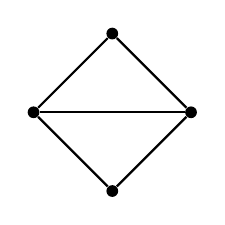
\begin{tikzpicture}
\node[shape=circle,fill=black,inner sep=1.5] (1) at (0,0) {};
\node[shape=circle,fill=black,inner sep=1.5] (2) at (-1,1) {};
\node[shape=circle,fill=black,inner sep=1.5] (3) at (1,1) {};
\node[shape=circle,fill=black,inner sep=1.5] (4) at (0,2) {};
\draw[thick] (1)--(2)--(4)--(3)--(1);
\draw[thick] (2)--(3);
\end{tikzpicture}
\end{center}
\item How many spanning trees does $G$ have?
\item How many acyclic orientations does $G$ have?
\item Compute the Tutte polynomial of the following graph $H$:
\begin{center}
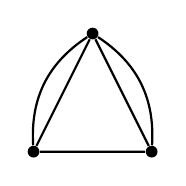
\begin{tikzpicture}[scale=1.5]
\node[shape=circle,fill=black,inner sep=1.5] (1) at (0,0) {};
\node[shape=circle,fill=black,inner sep=1.5] (2) at (1,0) {};
\node[shape=circle,fill=black,inner sep=1.5] (3) at (0.5,1) {};
\draw[thick] (1)--(2)--(3)--(1);
\draw[thick] (1) to[bend left] (3);
\draw[thick] (2) to[bend right] (3);
\end{tikzpicture}
\end{center}
\item How many spanning trees does $H$ have?
\item How many acyclic orientations does $H$ have?
\end{enumerate}


\end{document}
